\chapter{The limits of reconstruction, looked at again}\label{ch:limits}

Chapter~\ref{ch:floor} gave one number for the limit: the lost-band floor, 34.5\% at 3\um. The review showed that this
one number hides three different things. This chapter separates them. It is the most important chapter for
understanding what any score in this project means.

\section{Three bands instead of one floor}

Think of the 0.5\um\ field as a sum of ripples, each with a spatial frequency $k$ (in rad/\um). Fine detail is high $k$.
The blur multiplies each ripple by $H(k)=e^{-k\,\Delta z}$, so fine detail is damped most. Sort the ripples into three
bands:

\begin{center}
\small
\begin{tabularx}{\textwidth}{>{\raggedright\arraybackslash}p{2.6cm}>{\raggedright\arraybackslash}p{3.1cm}X}
\toprule
Band & Frequencies & What it is \\
\midrule
\textbf{Measured band} & below $k_c$ & The blurred signal is still stronger than the noise. A method only has to undo
the blur. \\
\textbf{Prior band} & from $k_c$ to $k_n$ & The signal has sunk below the noise in the measurement, but the target there is
real field: wire edges. Only a method that \emph{knows what sources look like} can fill it in. \\
\textbf{Noise band} & above $k_n$ & The target itself is mesh noise here. No method can reproduce it, and none should. \\
\bottomrule
\end{tabularx}
\end{center}

\begin{figure}[H]
\centering
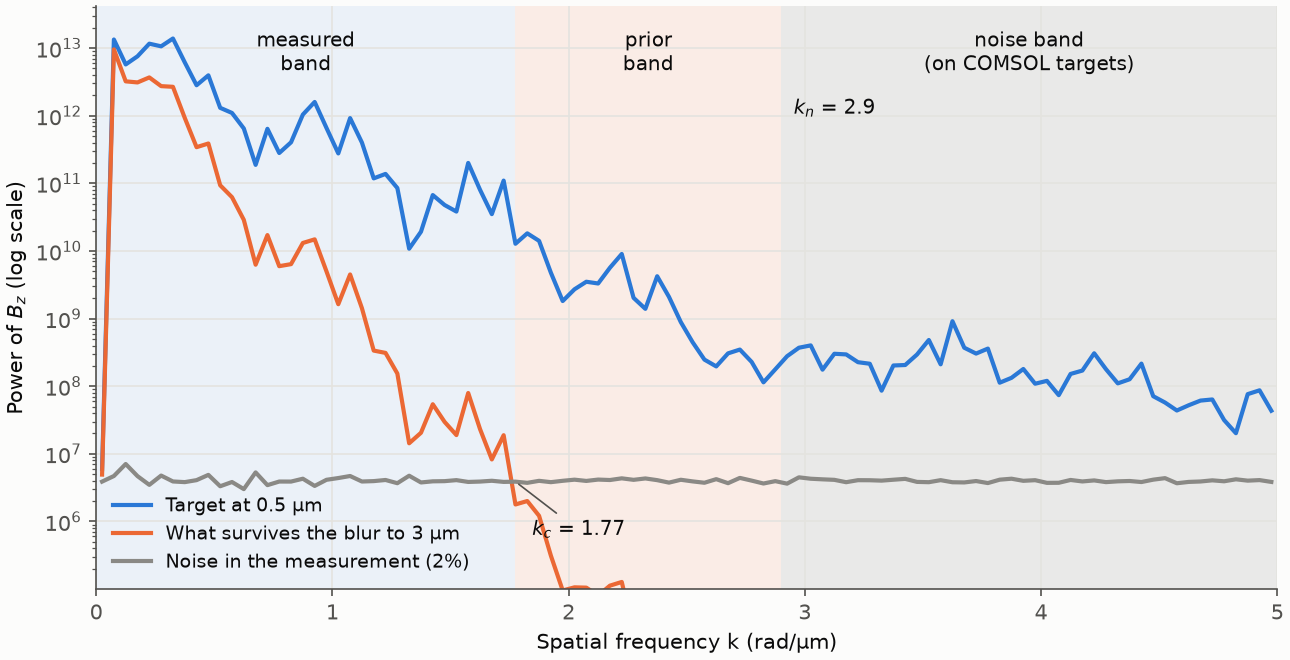
\includegraphics[width=0.88\textwidth]{late_bands}
\caption{The three bands on a simulated layout at 3\um\ to 0.5\um. Blue: power of the target. Orange: what survives the
blur. Grey: the noise level. Where orange drops below grey ($k_c$), the measurement stops carrying information.}
\label{fig:late_bands}
\end{figure}

On the 15 COMSOL pairs, measured as a share of the target's norm:
\begin{center}
\begin{tabular}{lccc}
\toprule
 & Measured band & Prior band & Noise band \\
\midrule
Share of the target's norm & 93.0\% & 32.9\% & 15.7\% \\
\bottomrule
\end{tabular}
\end{center}
These add as squares, not as plain numbers: $93.0^2+32.9^2+15.7^2\approx100^2$. That rule matters, and it comes back
below.

\section{The first edge, $k_c$: where signal sinks below noise}

$k_c$ is the frequency where the blurred signal and the noise are equally strong. The code walks up in steps of
0.05\,rad/\um\ and stops at the first step where the noise wins:

\begin{code*}{m12_common.py}
    h = np.exp(-k * dz)
    sig = np.abs(h * fs) ** 2
    res = np.abs(fb - h * fs) ** 2
    for a in np.arange(0, 8, 0.05):
        m = (k >= a) & (k < a + 0.05)
        if sig[m].sum() < res[m].sum():
            return float(a)
\end{code*}

Here \code{fs} is the spectrum of the sharp target and \code{fb} that of the measured input. \code{sig} is the power the
blur lets through. \code{res} is whatever in the measurement the blur model cannot explain, which is the noise. At
3\um\ on COMSOL, $k_c$ is between 1.0 and 1.6\,rad/\um.

\begin{careful}
$k_c$ uses the true target. So the band split is a way to \emph{diagnose} a method afterwards. It is not something a
method could use while reconstructing.
\end{careful}

\section{The second edge, $k_n$: where the target becomes noise}

How can we tell noise from field in the target, when we have no cleaner target to compare with? With physics. The
three components $B_x$, $B_y$, $B_z$ are not three independent images.

Above the sources there is no current, so the field can be written as the slope of one scalar function,
$\mathbf{B}=-\nabla\Phi$, and that function decays upward as $e^{-kz}$. Take the slope in each direction and the three
components at frequency $(k_x,k_y)$ become
\[
B_x=-i k_x\,\Phi,\qquad B_y=-i k_y\,\Phi,\qquad B_z=k\,\Phi .
\]
\textbf{One number $\Phi$ fixes all three.} In the component frame of our files (COMSOL's export is turned by a quarter
turn, Chapter~\ref{ch:comsol}) the same statement reads
\[
B_x=\frac{k_y}{k}\,\varphi,\qquad B_y=-\frac{k_x}{k}\,\varphi,\qquad B_z=i\,\varphi .
\]
So at each frequency, a real field is one complex number $\varphi$ times the fixed direction
$u=(k_y/k,\;-k_x/k,\;i)$. Mesh noise has no reason to point along $u$. The test is therefore: project the three measured
numbers onto $u$, and call the rest inconsistent.

\begin{code*}{m12_common.py}
    ux, uy, uz = ky / safe, -kx / safe, 1j * np.ones_like(k)
    phi = (np.conj(ux) * spectrum[0] + np.conj(uy) * spectrum[1] + np.conj(uz) * spectrum[2]) / 2
    out = np.stack([ux * phi, uy * phi, uz * phi])
\end{code*}

The division by 2 is the squared length of $u$: $(k_y^2+k_x^2)/k^2+1=2$. So \code{phi} is the least-squares best
$\varphi$, and \code{out} is the part of the field that one current sheet could have produced.

Now sum, in rings of width 0.1\,rad/\um, the total energy and the inconsistent energy of the five 0.5\um\ targets:

\begin{code*}{m12_common.py}
        r = f - sheet_consistent(f, kx, ky, k)
        idx = np.digitize(k, edges) - 1
        ok = (idx >= 0) & (idx < len(total))
        total += np.bincount(idx[ok], (np.abs(f) ** 2).sum(0)[ok], len(total))
        bad += np.bincount(idx[ok], (np.abs(r) ** 2).sum(0)[ok], len(total))
\end{code*}

The rule, fixed before any prediction was scored: $k_n$ is the first ring above 1\,rad/\um\ where more than half of the
energy is inconsistent.

\begin{code*}{m12_common.py}
    frac = bad / np.maximum(total, 1e-300)
    for edge, f in zip(lower, frac):
        if edge >= k_min - 1e-9 and f > share:
            return float(edge)
\end{code*}

\begin{center}
\begin{tabular}{lc}
\toprule
Frequency (rad/\um) & Inconsistent share of the targets' energy \\
\midrule
0.3 to 1.7 & below 3\% \\
1.9 to 2.4 & 14 to 31\% \\
\textbf{2.9} & \textbf{first above 50\%} \\
3 to 12 & 42 to 61\% \\
\bottomrule
\end{tabular}
\end{center}

So $k_n=2.9$\,rad/\um. Why is the share only about a half, and not 100\%, where it is all noise? Because noise is random
in three directions and the test removes two of them. Pure independent noise gives a share of about $2/3$.

\begin{keyidea}[A second, independent confirmation]
Chapter~\ref{ch:comsol} has COMSOL fields of the same coil on two different meshes. Above 2.9\,rad/\um\ they differ from
each other by a factor of 1.4, which is $\sqrt2$: exactly what two independent noise images give. Two unrelated
methods put the edge at the same place.
\end{keyidea}

\begin{careful}[An honest correction]
The review first put the edge at 2.2\,rad/\um, chosen by eye, and wrote that ``18--20\% of every score is mesh noise''.
Both were wrong. The fixed rule gives 2.9. And the noise does not add 16 points to a score, as the next section shows.
\end{careful}

\section{Errors add as squares}

A method's error can be split by band in the same way as the target. The three parts add as squares:
\[
\text{raw}^2=\text{(measured-band error)}^2+\text{(prior-band error)}^2+\text{(noise-band error)}^2 .
\]
Every method outputs nothing sensible in the noise band, so its error there equals the target's own content, about
15.7\%. That is the same for everyone. Removing it:
\[
\sqrt{30.5^2-15.6^2}\approx26.2\%,\qquad \sqrt{24.3^2-15.9^2}\approx18.4\% .
\]
So the noise band lifts a raw score by about 4 to 6 points, not by 15.7. And because it is added in squares to every
method, it \emph{squeezes the differences between methods}. Two methods that are 6 points apart in raw score are 8
points apart once the shared noise is removed.

\section{Scoring four ways}

From here on every method is scored four ways: raw, against the target with the noise band cut off (``low-passed''), in
the measured band alone, and in the prior band alone. All four come from one function. Its core:

\begin{code*}{m12_common.py}
        def band(mask, a):
            return float(np.sqrt((np.abs(a) ** 2)[mask].sum() / n_pix) / norm)
        low = k < k_noise
\end{code*}

\begin{code*}{m12_common.py}
            in_band=band(k < kc, err), prior_band=band((k >= kc) & (k < k_noise), err),
            noise_band=band(k >= k_noise, err), k_c=kc,
\end{code*}

\code{err} is the spectrum of (output minus target). \code{band} keeps only the frequencies in the mask and measures
what is left, as a fraction of the whole target.

\begin{center}
\footnotesize
\setlength{\tabcolsep}{4pt}
\begin{tabular}{lccccc}
\toprule
COMSOL, 3\um\ to 0.5\um & Raw & Low-passed & Measured & Prior & Noise \\
\midrule
Target's own content & & & 93.0\% & 32.9\% & 15.7\% \\
\midrule
MAGIC-UNet run 2 + correction (Ch.~\ref{ch:consistency}) & 24.3\% & 18.5\% & 11.0\% & 14.6\% & 15.9\% \\
FISTA, 1{,}000 iterations (Ch.~\ref{ch:fista_depth}) & 26.7\% & 21.9\% & 9.1\% & 19.3\% & 15.6\% \\
MAGIC-UNet run 2 & 27.0\% & 22.0\% & 16.0\% & 14.6\% & 15.9\% \\
FISTA, 300 iterations & 30.5\% & 26.4\% & 9.6\% & 23.8\% & 15.6\% \\
FISTA-Net run 2 & 33.3\% & 29.5\% & 13.3\% & 25.6\% & 16.2\% \\
CSC-LISTA strict, 64 layers & 33.8\% & 30.2\% & 12.3\% & 26.7\% & 15.6\% \\
Tikhonov, $\mu=0.0316$ & 49.3\% & 47.4\% & 33.8\% & 32.0\% & 15.7\% \\
\bottomrule
\end{tabular}
\end{center}

\begin{keyidea}[How to read this table: it is the whole project in seven rows]
\begin{itemize}
\item \textbf{Noise band:} about 15.7\% for everyone. Nobody can change it.
\item \textbf{Tikhonov} leaves the whole prior band untouched: its error there (32.0\%) is the target's content (32.9\%).
A linear filter invents nothing.
\item \textbf{The unrolled networks} recover a little of the prior band (26--27\% left of 32.9\%). They behave almost like
linear filters. That is why they sat next to the Wiener oracle.
\item \textbf{FISTA} recovers more the longer it runs: 23.8\% at 300 iterations, 19.3\% at 1{,}000.
\item \textbf{MAGIC-UNet} recovers the most: 14.6\%. This is where a prior on the \emph{current} pays off.
\item \textbf{But in the measured band MAGIC-UNet is the worst of the good methods} (16.0\% against FISTA's 9.1\%). It wins
where the data are silent and loses where the data speak. Chapter~\ref{ch:consistency} fixes exactly this.
\end{itemize}
\end{keyidea}

\section{What the old floor really was}

The lost-band floor of Chapter~\ref{ch:floor} was: delete everything above $k_c$ from the true target and measure the
error. That deletes the prior band \emph{and} the noise band together: $\sqrt{32.9^2+15.7^2}\approx36\%$. So about a third
of the target lies above $k_c$, as Chapter~\ref{ch:floor} said. But it is two different thirds:
\begin{itemize}
\item the prior band is real and recoverable with the right prior. It is where methods differ;
\item the noise band is a fixed cost that says nothing about any method.
\end{itemize}
And these numbers belong to COMSOL's mesh noise. A real QDM has photon noise with another level and another spectrum,
so $k_c$ and the floor will be different there.

\begin{careful}[Do not carry 34.5\% into a paper]
It is a property of this data set, not of the physical problem.
\end{careful}

\section{The height ambiguity is one-sided}

Chapter~\ref{ch:question} showed that a source at depth $h$ and a sharper source at depth $h+\delta$ give the same
field, and concluded that the height cannot come from the field alone. The review sharpened this.

Go \textbf{deeper} by $\delta$: the source must be sharper by $e^{k\delta}$, a factor that grows without limit with $k$.
A real wire of width $w$ has a spectrum that falls off only slowly (like $\sin(kw/2)/(kw/2)$). Multiply a slowly falling
spectrum by a growing exponential and the result blows up: the source would need infinite energy. So a hypothesis that
is too deep produces a source that \emph{rings} wildly.

Go \textbf{shallower} by $\delta$: the source must be smoother by $e^{-k\delta}$. A smoother current is always a perfectly
reasonable current.

\begin{keyidea}[What this gives]
With no prior at all, every depth \emph{up to} the true one is possible, and no depth beyond it. The true depth is the
deepest hypothesis whose source stays finite. This is sharper than ``impossible'', and it says what an estimator
should do: push the depth down until the source starts to ring.
\end{keyidea}

Three practical consequences:
\begin{itemize}
\item \textbf{Noise blurs the bound.} Only frequencies below $k_c$ are seen, so two depths that differ by less than about
$1/k_c$ are hard to separate. At 3\um, $k_c\approx1.1$\,rad/\um\ gives about 1\um. The uncertainty should grow roughly in
proportion to the standoff.
\item \textbf{Height trades against wire width and thickness.} A conductor of thickness $t$ changes the spectrum by
roughly $e^{-kt/2}$, which is almost exactly a shift in height. So what can be estimated is an \emph{effective}
standoff. A network trained on wires 1.6--3.2\um\ wide has learned those widths, and a reviewer will test it on a
0.5\um\ or a 6\um\ wire.
\item \textbf{Knowing the drive current does not help by itself,} but together with a wire model it does. That is how NV
groups calibrate their standoff on a known wire, and it is the route to ground truth on a real instrument.
\end{itemize}

\begin{defend}[If your professor asks: what is the real limit of this reconstruction?]
There are three. Below $k_c$ any good method works. Between $k_c$ and the noise edge the answer depends entirely on the
prior, and this is where methods differ: MAGIC-UNet leaves 14.6\% there, FISTA 19.3\%, a linear filter 32\%. Above the
noise edge the COMSOL target is noise, about 16\% of its norm, and no method can or should match it.
\end{defend}

\begin{defend}[If your professor asks: can the standoff be estimated from the image or not?]
Not from the image alone, but the ambiguity is one-sided: the data give an upper bound on the depth, because a source
placed too deep would need unbounded sharpness. A prior on what sources look like turns that bound into an estimate,
with a resolution of about $1/k_c$, roughly a third of the standoff here.
\end{defend}
